\documentclass{article}
\usepackage{graphicx}
\usepackage[french]{babel}
\usepackage[utf8]{inputenc}

\usepackage{lastpage}
\usepackage{fancyhdr}
\usepackage[a4paper]{geometry}
\geometry{hscale=0.7,vscale=0.75,centering}

\pagestyle{empty}
\pagestyle{fancy}

\makeatletter
%En-Tête
\fancyhf{}
\lhead{\@school}
\chead{\@headTitle}
\rhead{\@entreprise}
\lfoot{\@author}
\rfoot{\raggedleft \thepage/\pageref{LastPage}}
%Page de garde
% Une commande semblable à \rlap ou \llap, mais centrant son argument
\def\clap#1{\hbox to 0pt{\hss #1\hss}}%
% Une commande centrant son contenu (à utiliser en mode vertical)
\def\ligne#1{%
  \hbox to \hsize{%
    \vbox{\centering #1}}}%
% Une commande qui met son premier argument à gauche, le second au 
% milieu et le dernier à droite, la première ligne de chacune de ces
% trois boites coïncidant
\def\haut#1#2#3{%
  \hbox to \hsize{%
    \rlap{\vtop{\raggedright #1}}%
    \hss
    \clap{\vtop{\centering #2}}%
    \hss
    \llap{\vtop{\raggedleft #3}}}}%
% Idem, mais cette fois-ci, c'est la dernière ligne
\def\bas#1#2#3{%
  \hbox to \hsize{%
    \rlap{\vbox{\raggedright #1}}%
    \hss
    \clap{\vbox{\centering #2}}%
    \hss
    \llap{\vbox{\raggedleft #3}}}}%
% La commande \maketitle
\def\maketitle{%
  \thispagestyle{empty}\vbox to \vsize{
  	\haut{\includegraphics[scale=\@logoSchoolScale]{\@logoSchool}}
  		 {}
  		 {\includegraphics[scale=\@logoEntrepriseScale]{\@logoEntreprise}}
    \vfill
    \haut{\hspace{2cm}}{\Large \@title}{\hspace{2cm}}
    \vspace{5mm}
    \ligne{\Large \@entreprise}
    \vspace{1mm}\ligne{\texttt{\@stageDate}}
    \vfill
    \ligne{Réalisé par : \@author}
    \ligne{Tuteur : \@tutor}
    \ligne{Maître de stage : \@supervisor}
    \vspace{5mm}
    \bas{}{\@location, \@date}{}
    }
  \cleardoublepage
}
% Les commandes permettant de définir la date, le lieu, etc.
\def\date#1{\def\@date{#1}}
\def\entreprise#1{\def\@entreprise{#1}}
\def\title#1{\def\@title{#1}}
\def\location#1{\def\@location{#1}}
\def\stageDate#1{\def\@stageDate{#1}}
\def\author#1{\def\@author{#1}}
\def\tutor#1{\def\@tutor{#1}}
\def\supervisor#1{\def\@supervisor{#1}}
\def\logoSchool#1{\def\@logoSchool{#1}}
\def\logoSchoolScale#1{\def\@logoSchoolScale{#1}}
\def\logoEntreprise#1{\def\@logoEntreprise{#1}}
\def\logoEntrepriseScale#1{\def\@logoEntrepriseScale{#1}}
\def\school#1{\def\@school{#1}}
\def\entreprise#1{\def\@entreprise{#1}}
\def\headTitle#1{\def\@headTitle{#1}}
% Valeurs par défaut
\date{\today}
\entreprise{}
\title{}
\location{}
\stageDate{}
\author{}
\tutor{}
\supervisor{}
\logoSchool{}
\logoEntreprise{}
\logoSchoolScale{1}
\logoEntrepriseScale{1}
\school{}
\entreprise{}
\headTitle{}

\makeatother

%Valeurs à remplacer
\title{Plateforme de tests pour une infrastructure d'intégration continue}
\entreprise{Thales Corporate Services}
\stageDate{6 juin 2011 - 2 septembre 2011}
\author{Hugo Wood}
\tutor{Julien Allali, Responsable des seconde année à l'ENSEIRB-MATMECA}
\supervisor{Jérôme Vacher, Integration and Code Building Manager à Thales Corporate Services}
\location{Californie}
\logoSchool{logo_enseirb.png}
\logoSchoolScale{0.3}
\logoEntreprise{logo_thales.jpg}
\logoEntrepriseScale{0.3}
\school{ENSEIRB}
\headTitle{Rapport de stage de 2\up{ème} année}

\begin{document}

\maketitle


\tableofcontents
\newpage

\section{Remerciements}

J'aimerais remercier messieurs Jérôme Vacher et Boris Chevalier pour m'avoir 
donner l'opportunité d'effectuer ce stage, ainsi que tous les membres des 
équipes ThalesControl et IVV pour leur acceuil chaleureux : Grégory Boissinot, 
Phillipe Chevalier, François Gaillot-Drevon, Frédéric Grandisson, Robin Jarry, 
et Aravindan Mahendran. Je voudrais remercier également tout particulièrement 
mon coéquipier stagiaire Antonin Morelle, dont la présence a rendu ce stage 
plus intéressant et constructif.

Merci à Jérôme Vacher pour sa lecture constructive de ce rapport.
\newpage

\section{Introduction}

Ce rapport regroupe les informations concernant mon stage industriel effectué
entre ma seconde et troisième année d'école d'ingénieur, au sein de l'entreprise
Thales Corporate Services (abbrégée CST, maintenant Thales Global Services), une
filiale du groupe Thales.

Postuler pour ce stage est venu de mon désir de travailler au sein d'un grand 
groupe, en espérant faire partie d'une équipe travaillant sur un produit utilisé
par un relatif grand nombre d'utilisateur. Thales Corporate Services développe 
des logiciels destinés à être utilisé par l'ensemble du groupe Thales, ce qui
représente effectivement un large ensemble d'utilisateurs.

Ce stage à orientation technique a eu pour objectif de poursuivre les travaux 
d'un précédent stagiaire sur une plate-forme de test pour un des produits de la
firme. Le dit produit ainsi que le processus qui permet de le tester est 
détaillé dans la partie \ref{ThalesControl}. La plate-forme de test elle-même 
est donc essentiellement un outils d'aide au développement pour l'équipe 
derrière le produit final, avec laquelle j'ai travaillé en étroite 
collaboration.

Dans ce rapport, je vais d'abord présenter l'entreprise Thales Corporate 
Services, son rôle au sein de Thales ainsi les enjeux des projets sur lesquelles
elle travaille. Je poursuivrais ensuite avec ma mission technique, ses 
objectifs à sa réalisation.
\newpage

\section{Le groupe Thales et la filiale Thales Corporate Services}

\subsection{Thales}

Thales est un leader mondial des hautes technologies pour les marchés de 
l’aéronautique et de l’espace, de la défense, de la sécurité et des transports, 
disposant d’environ 68 000 collaborateurs dans 50 pays, en France, aux 
Etats-Unis, en Amérique latine, Corée du sud et Australie. Le succès du groupe 
s'explique par sa capacité à développer des systèmes critiques multidomestiques,
un potentiel humain exceptionnel avec un haut niveau de qualification (60\% 
d’ingénieurs et cadres), des équipes multiculturelles unies par les mêmes 
valeurs et une politique de ressources humaines dynamique. Le chiffre d'affaire
du groupe est de 12.8 milliards d'euros en 2009. Les actions sont principalement
partagés entre l'état français à 27\% et Dassault Aviation à 26\%, le reste étant 
flottant.

Thales est composé de sept divisions : Systèmes de défense et sécurité, 
Opérations Aériennes, Avionique, Espace, Systèmes de mission de défense, 
Défense Terrestre, Systèmes de Transport.
Chacune de ces divisions est spécialisée dans des domaines définis par leurs 
marchés. L’entreprise dispose en plus de six directions spécialisées dans les 
fonctions transverses au groupe Thales que sont : Finance et Juridique, 
Recherche et Technologie, Opérations, Audit Interne, Stratégie, Ressources 
Humaines et Communications. Ces directions sont parfois décentralisées par pôle 
ou région du monde.

\subsection{Thales Corporate Services}

Thales Corporate Services (Thales CST ou simplement CST) est
sous la responsabilité de la direction des Opérations. C’est une filiale à 100\%
de Thales, comptant 293 employés. Il s'agit d'une entité regroupant un ensemble 
de compétences, de ressources et de moyens afin de mettre en oeuvre des services
partagés entre les entités du groupe. Dans le cadre de ses missions, Thales CST 
fournit aux entités du groupe des services appartenant à des domaines tels que :
l'"engineering" des systèmes, des logiciels et du matériel, les processus et 
méthodologies associés, le développement de solutions pour les systèmes 
d’information (infrastructure et applications) et services associés (déploiement
des solutions, pilotage des contrats de services, etc.) ainsi que les achats 
transverses. Le déploiement de ces processus et outils communs dans les 
différents pays et/ou dans les entités du groupe s’appuie sur les moyens propres
à chaque pays et/ou entités. En fonction de la stratégie de déploiement adoptée,
Thales CST interviendra afin de supporter les pays et/ou entités dans le 
déploiement de ces processus et outils communs. Les objectifs de Thales CST 
sont : la qualité des services et des produits, la tenue des engagements en 
termes de délais et de maîtrise des coûts, l’amélioration de la compétitivité du
groupe en s’appuyant sur la mutualisation des moyens.

Pour mener à bien ses missions, Thales CST est organisée en centres de 
compétences qui répondent chacun à des règles de gouvernance qui leur sont 
propres. Un centre de compétences peut fournir : 
\begin{itemize}
	\item{des services récurrents qui s’appliquent à l’ensemble des unités d’un 
	pays (achats généraux) ou à l’ensemble des unités du groupe;}
	\item{le développement de projets transverses qui intéressent plusieurs 
	unités/divisions du groupe;}
	\item{des compétences qui participeront au développement de projets dans le 
	domaine des systèmes d’information du groupe.}
\end{itemize}

Thales CST est organisée en trois centres de compétences : 

\begin{description}
\item[Purchasing] qui est placé sous l’autorité opérationnelle de la Direction 
des Achats du Groupe. Il comprend : des activités couvrant les achats indirects 
en France et liées à la mise en oeuvre de contrats et accords cadres, de 
politiques fournisseurs et les approvisionnements associés, des activités liées 
aux initiatives achats transverses au Groupe (mise en oeuvre de contrats et 
accords cadres, de politiques fournisseurs) couvrant les segments achats directs
(inclus dans les offres de Thales).
\item[Information Systems \& Process (IS\&P)] qui est placé sous l’autorité 
opérationnelle de la Direction des Systèmes d’Information du Groupe. Il 
comprend : les activités de management de la production des services 
informatiques pour le compte des unités du Groupe en France ainsi que le 
management de la production des services d’infrastructure du Groupe au niveau 
mondial, la mise à disposition de compétences en matière de conception, de 
développement et de support au déploiement des systèmes d’information et des 
infrastructures communes à plusieurs unités du Groupe.
\item[Engineering \& Process Management (EPM)] qui est chargé d’accroître la 
compétitivité des entités du groupe Thales en fournissant des solutions 
optimisées sur l’ensemble du cycle de développement des produits et systèmes. 
EPM fournit dans ce but des procédés, méthodes et des outils.
\end{description}

Mon stage s'est déroulé au sein de EPM, et plus précisément dans la département 
System \& Software, qui fournit les logiciels de développement pour les entités 
Thales à travers le monde. 

\subsection{Thales Global Services}

En août 2011, Thales Corporate Services a changé de nom et est devenu Thales Global Services. 
Ce changement fait partie d'un processus de plus grande ampleur visant à 
regrouper tous les services transverses de Thales, et en particulier la 
communication, le marketing et les ressources humaines, tout ceci au niveau 
mondial. La transformation devrait se traduire par une expansion majeure 
du centre IS\&P et par une augmentation du nombre d'employés, qui devrait 
avoisiner les 800 (contre moins de 300 actuellement) dans le courant 2012.
\newpage

\section{Contexte du stage}

Afin de bien comprendre le sujet de mon stage, il est indispensable d'assimiler 
l'environnement logiciel dans lequel il se positionne, et le problème rencontré 
par les équipes de EPM qui a conduit à la production du programme que j'ai 
écrit.

\subsection{L'intégration continue}

L'intégration continue est un ensemble de pratiques utilisées en génie logiciel.
Elles consistent à vérifier à chaque modification de code source que le résultat
des modifications ne produit pas de régression de l'application en cours de 
développement. L'intégration continue se met en place grâce à deux blocs 
principaux :
\begin{description}
	\item[Source Control Manager (SCM)], qui permet aux développeurs de partager
	le code source d'un projet en le centralisant sur un dépôt. Dans le cadre de
	l'intégration continue, il est indispensable que les programmeurs livrent 
	leur code sur le dépôt très fréquemment. Parmi les SCM les plus connus, on
	trouve Subversion, Git et Mercurial. Thales CST utilise ClearCase.
	\item[Continuous Integration Scheduler/Server], qui intérroge régulièrement 
	le dépôt 
	de source. Si il y a eu modification depuis la dernière compilation, le 
	serveur d'intégration continue lance une nouvelle compilation, les tests 
	associés, et toute autre tâche qui lui a été demandée d'effectuer sur le 
	code en question. Si un problème est détecté, les développeurs sont alertés.
	Exemples de serveur CI: CruiseControl, Hudson, Jenkins, Buildbot, Apache 
	Continuum.
\end{description}

L'intérêt de l'intégration continue est la réactivité qu'elle alloue 
aux développeurs. En effet, avec un processus bien en place, ceux-ci peuvent 
être mis au courant d'une multitude de problèmes provenant du code source, 
au jour le jour, ce qui évite à des bogues de rester dans l'application trop 
longtemps. Du temps et de l'argent est ainsi sauvegardé.

L'intégration continue est donc un outils de contrôle qualité extrêmement 
puissant. De plus, les serveurs prennent généralement en charge des extensions, 
ce qui les rend flexibles et compatibles à de nombreux contextes de 
développement.

\subsection{Qualité du code}

Contrôler la qualité d'un code source consiste à vérifier qu'il vérifie un 
certain nombre de critères. Ces critères peuvent par exemple être: respecter des
conventions syntaxiques, contenir un certain pourcentage de commentaires, 
minimaliser la complexité par fonction ou par classe, être couvert par des tests
unitaires. Des outils d'analyse de code existent afin d'extraire ces 
informations et de les rendre présentables à l'utilisateur. Ces outils sont 
aussi utiles pour les développeurs que pour les chefs de projet, qui peuvent 
ainsi suivre les progrès du projet à l'aide d'une interface attrayante.

Cette technique de qualité peut être couplée avec l'intégration continue de 
manière très intéressante puisque le serveur d'intégration continue peut 
lancer automatiquement les analyses de code voulues et livrer les rapports 
correspondant là où ils sont désirés.

\begin{figure}[htb]
	\centering
	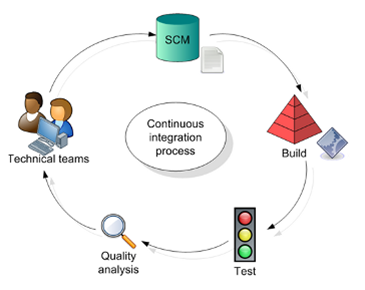
\includegraphics{continuous_integration.png}
	\caption{Le processus d'intégration continue couplé à l'analyse qualité}
\end{figure}

\subsection{ThalesControl}
\label{ThalesControl}

Afin d'améliorer la compétitivité des entités Thales, EPM développe au sein 
de l'équipe Code Building une 
solution d'intégration continue clé en main, appelée ThalesControl. Elle couple 
un serveur d'intégration continue, Hudson, et un aggrégateur de métriques de 
qualité, Sonar. Ces logiciels ne sont pas développés par Thales, et sont 
libres et gratuits. Le travail de Thales CST sur ThalesControl consiste à assurer 
une compatiblité parfaite entre les logiciels au fur et à mesure de leurs
mises à jour respectives. Le second objectif de ThalesControl est de s'adapter
à toutes les entités, qui utilisent des outils de développement très variés. 
Thales CST ajoute donc à Hudson et Sonar une multitude d'extensions pour l'un et
pour l'autre, afin qu'ils prennent en charge différents SCM, moteur de 
production (Make, Gradle, Maven, Ant...), plate-formes de test (xUnit), langages
de programmation, ou autres composants de la chaîne de construction de 
l'application cible. Chaque extension à sa propre progression. Certaines sont 
développées par la communauté libre, d'autres par Thales CST, d'autres encore 
par des entités Thales différentes. L'équipe ThalesControl doit donc jongler 
avec toutes ces briques logiciels (environ 80) dont les versions changent 
sans cesse, regrouper un ensemble qui fonctionne, et livrer le résultat.

ThalesControl est hautement personnalisable : il est possible d'installer ou non
un composant et de choisir la version de chaque composant.

\begin{figure}[htb]
	\centering
	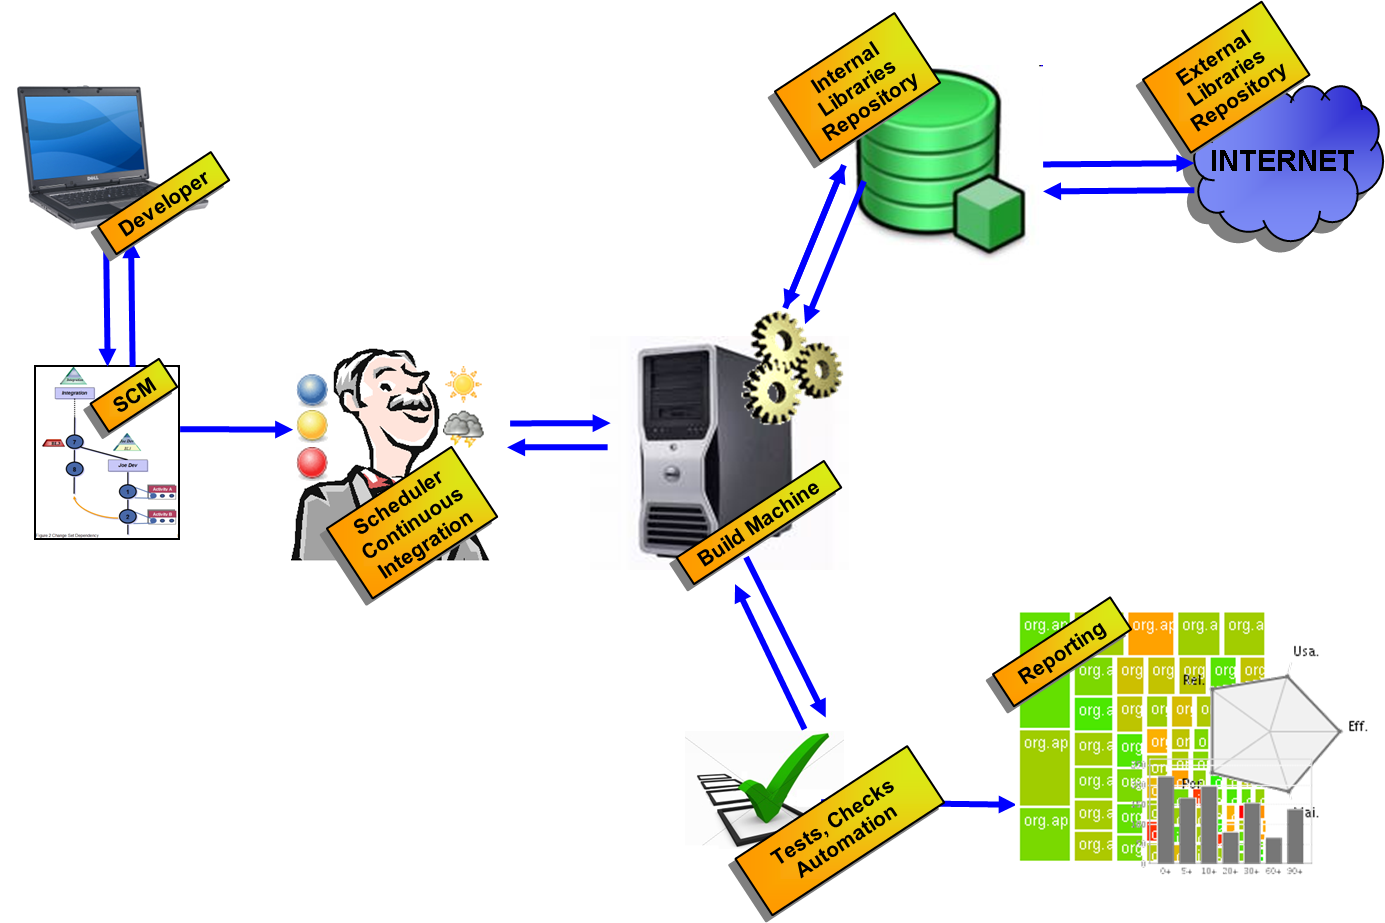
\includegraphics[scale=0.5]{continuous_integration_with_thales_control.png}
	\caption{L'intégration continue avec ThalesControl}
\end{figure}

Additionnellement, ThalesControl est fourni avec un installateur qui installe et
configure tous les composants selon les désirs de l'utilisateur. Ces désirs 
doivent être spécifiés dans un fichier de configuration écrit à l'avance.

On peut remarquer ici que l'équipe ThalesControl utilise de nombreux programmes libres. 
J'aimerais préciser que l'entreprise ne se contente pas d'utiliser ces 
logiciels, mais participe activement à leur développement, notamment par le 
biais d'extensions, que Thales met généralement sous licence libre 
et à disposition de la communauté. Cette philosophie, défendue par Jérôme Vacher,
est justifiée par le fait que Thales CST est un centre de coût pour Thales, et
n'a pas vocation à générer de profits.  Elle ne peut donc que tirer avantage 
de la communauté open-source, qui présente une source d'idées et de testeurs, 
ainsi que, parfois, de développeurs. C'est donc un moyen de réduire les coûts.

\subsection{La problématique Hudson/Jenkins}
\label{Hudson_Jenkins}

La communauté autour de Hudson a vu d'un mauvais {\oe}il le rachat de Sun 
Microsystems, détenteur des droits d'exploitation du nom Hudson et développeur 
originel du projet, par Oracle en 2010. Après des négociations non-abouties 
entre la dite communauté et Oracle, la première a décidé de créer une nouvelle 
branche du projet n'étant pas sous le contrôle d'Oracle. Le nouveau logiciel 
ainsi né a été nommé Jenkins. Oracle a de son côté conservé Hudson, puis l'a 
donné à la Fondation Eclipse, organisation majeure du monde du logiciel libre. 
Les deux logiciels cohabitent à présent, et sont tout deux activement développés.

Ces évènements impactent évidemment ThalesControl puisque l'équipe doit choisir 
quelle branche suivre. Durant mon stage, aucune décision finale n'a été prise.
La prochaine version de ThalesControl devait être livrée avec la version de 
Hudson distribuée juste avant la séparation, vieille de plusieurs mois.

Le problème est que la plupart des extensions avait déjà fait leur choix et 
nombre d'entre elles étaient déjà disponibles pour la dernière version de 
Jenkins. L'équipe de ThalesControl se voyait donc dans l'obligation, pour se 
maintenir à jour et pour répondre aux demandes de ses utilisateurs, d'essayer 
de fournir des extensions Jenkins avec Hudson. Tester à la main chacune des 
extensions et éventuellement les modifier pour les rendre compatibles est un 
travail trop important.

Le besoin d'un outil de test de compatibilité automatique entre serveur 
d'intégration et extensions est alors devenu critique.

\subsection{La problématique Sonar}
\label{ProbSonar}

Sonar est mis à jour très régulièrement. Une mise à jour majeure voit le jour 
environ tous les 3 mois. Ces mises à jour cassent souvent l'interface de 
programmation des extensions pour Sonar. Cela veut dire qu'à chaque nouvelle 
version, les développeurs des extensions doivent modifier leur code. Thales 
CST a créé une extension pour Sonar 2.0, mais n'a pas les 
ressources pour la maintenir. Ainsi pendant plus d'un an ThalesControl a été 
livré avec Sonar 2.0 alors que pendant ce laps de temps 7 versions de Sonar sont 
sorties.

Sous la pression des utilisateurs, Thales CST a du allouer du temps et des 
ressources à la migration de Sonar 2.0 à Sonar 2.8 (puis 2.9 et 2.10, sorties 
rapidement après). La problèmatique principale a été de trouver un moyen 
d'implémenter les mêmes fonctionnalités que l'extension pour Sonar 2.0, 
mais d'une manière requierant moins de maintenance à chaque nouvelle version de 
Sonar.

Durant ce processus, l'équipe ThalesControl a examiné plusieurs solutions et a 
pour cela du étudier Sonar de plus près. En particulier, l'organisation de la 
base données de Sonar ainsi que les modifications qui lui sont apportées entre 
chaque nouvelle version ont été observées. Le besoin s'est alors fait sentir 
de posséder un outils capable de comparer des bases de donneés et de fournir 
un résultat lisible et exploitable.

\subsection{La solution TCtest}
\label{TCtest}

\subsubsection{Objectif}

Afin de délester le personnel des tâches répétitives de test d'intégration 
entre les composants de ThalesControl, il a été décidé de développer un outil 
automatisant au mieux ces tâches. Cet outil a été nommé TCtest. Un premier 
stagiaire, Francis Ngougo, 
a programmé un premier jet d'un tel programme pendant 6 mois fin 2010.
Il est important de préciser qu'un des objectifs 
de TCtest est d'être tout-terrain. C'est-à-dire qu'il doit être capable de :
\begin{itemize}
	\item{travailler avec n'importe quelle installation de ThalesControl, sachant que 
	celui-ci est constitué d'environ 80 composants dont la fréquence de renouvellement 
	est très rapide;}
	\item{travailler avec de multiples installations de ThalesControl en même 
	temps;}
	\item{permettre à l'utilisateur de créer de nouveaux jeux de tests sans 
	toucher au code source.}
\end{itemize}

\subsubsection{Vocabulaire}
\label{Voc}

\begin{description}
	\item[Service] Brique logiciel compilée en une librairie (un fichier JAR 
	dans le cas présent). Les services sont découverts et chargés dynamiquement 
	par TCtest. Les services effectuent généralement des tâches très simples.
	\item[Workflow] Synonymes de test, c'est-à-dire une séquence d'actions qui 
	produit généralement un résultat booléen (réussi ou non). Les workflows 
	sont définis par l'utilisateur dans des fichiers XML. Les actions en 
	questions sont effectuées par des services. Un workflow est donc une 
	séquence de services, avec éventuellement des paramètres pour chaque 
	service.
	\item[Instance de ThalesControl] Ensemble de composants (chacun associé
	à une version) formant un produit ThalesControl.
\end{description}

\subsubsection{Principe}

Je présenterai seulement succintement le logiciel
dans cette partie, et détaillerai au besoin dans la partie Réalisation. TCtest 
fonctionne suivant 4 étapes :
\begin{description}
	\item[Initialisation]{
	TCtest lit des fichiers de configuration écrit par l'utilisateur. Ces 
	fichiers décrivent premièrement l'environnement (dans quel dossier chercher 
	les tests disponibles, dans quel dossier installer ThalesControl...) et 
	deuxièmement quels tests (aussi appelés workflows) lancer, et sur quelles 
	instances de ThalesControl. La configuration fait référence à ces éléments 
	par le nom du dossier dans lequel trouver leur définition, sachant que ces
	définitions sont écrites en XML.}
	\item[Installation]{
	TCtest installe toutes les instances de ThalesControl qui lui sont demandées de 
	tester, grâce à l'installateur.}
	\item[Lancement]{
	TCtest lance les composants de ThalesControl qui requièrement un tel lancement 
	(Tomcat, Hudson, Sonar...).}
	\item[Test]{
	TCtest lit les définitions (fichiers XML) des tests qui lui sont demandés 
	d'effectuer puis exécute les tests. L'exécution comprend la lecture d'un fichier
	de workflow, l'instanciation puis l'exécution des services mentionnés dans ce 
	workflow.}
\end{description}

Je conseille fortement au lecteur intéressé de lire le manuel utilisateur (en 
Anglais) de TCtest 5.0, que j'ai écrit lors de mon stage. Le manuel se trouve en
annexe de ce rapport.

\subsubsection{Parallélisation}
\label{Parallel}

TCtest 1.0 est implémenté sous forme de pipeline. Les étapes d'installation, de 
lancement et de test sont chacune traitées par un thread différent. Les 3 threads 
prennent leurs entrées et mettent leurs sorties dans des files. Cela signifie 
qu'il est possible de tester une première instance pendant qu'une seconde 
s'installe. TCtest étant destiné à travailler sur de grandes batteries de tests,
ce processus a été mis en place pour gagner du temps.

\subsubsection{Modularité}

TCtest se décompose en plusieurs modules :
\begin{description}
	\item[Le lanceur]{C'est l'application principale, que l'on configure et que
	l'on lance pour effectuer les tests}
	\item[L'API]{C'est l'ensemble des interfaces et classes fournies aux 
	développeurs tiers afin qu'ils puissent étendre les fonctionnalités de 
	TCtest.}
	\item[Les services]{Voir \ref{Voc}.}
\end{description}

\newpage

\section{Objectifs de la mission technique}

Il n'y avait pas de cahier des charges précis et rédigé. Je pense que l'objectif
à mon arrivé pouvait se résumer à "il faut que TCtest puisse résoudre la 
problématique Hudson/Jenkins" (voir partie \ref{Hudson_Jenkins}). En détaillant 
un peu plus :

\begin{itemize}
	\item{prendre connaissance de ThalesControl, de ses composants principaux, 
	de sa procédure d'installation}
	\item{prendre connaissance de TCtest, son architecture, son implémentation, 
	son fonctionnement, des outils utilisés pour son développement}
	\item{améliorer TCtest
	\begin{itemize}
		\item{le rendre plus facile d'utilisation}
		\item{lui donner la capacité d'exploiter des instances de ThalesControl
		déjà installées et lancées}
		\item{étudier des cas d'utilisation donnés par les futurs utilisateurs
		et s'assurer qu'il est bien adapté à ceux-ci 
		(problématique Hudson/Jenkins en particulier)}
		\item{écrire des services supplémentaires, selon les besoins}
		\item{écrire un manuel utilisateur}
	\end{itemize}}
\end{itemize}
\newpage

\section{Réalisations}

Cette partie se constitue d'un ensemble de sous-parties décrivant chacune une 
modification que j'ai réalisées sur TCtest. L'ordre chronologique n'est pas 
respecté, en faveur d'un enchainement logique que j'espère plus facile à 
suivre. Par conséquent, ce qui est considéré ici comme une réalisation a pu 
s'écrire de manière itérative tout au long du stage.

Je précise que pendant la première moitié de mon stage, un autre 
stagiaire, Antonin Morelle, a travaillé avec moi sur le programme.

\subsection{Préambule : Technologies et concepts}

TCtest est écrit en Java et construit avec Maven. Eclipse a été utilisé comme 
éditeur. Le code source était géré avec IBM ClearCase et les tâches et bugs 
gérés avec JIRA. Les concepts abordés dans le logiciel sont les suivants :
\begin{itemize}
	\item{orienté-objet}
	\item{multi-threading}
	\item{programmation par interface}
	\item{chargement dynamique et exécution de code externe}
	\item{génération de classe à partir de schémas XML}
	\item{désérialisation d'objet depuis une source XML}
	\item{web services avec Jersey}
\end{itemize}

\subsubsection{JAXB}

JAXB est une API permettant de:
\begin{enumerate}
	\item{générer des classes à partir de schéma XML}
	\item{transformer des fichiers XML en instances de ces classes}
\end{enumerate}
JAXB est très utilisé dans TCtest. C'est un API très pratique puisqu'elle 
permet d'exploiter des données XML de manière très simple. Cependant elle 
est limité par le fait que les classes générées ne peuvent avoir aucun 
comportement. Elles ne contiennent que des accesseurs sur des attributs 
correspondant aux balises \verb|element| du schéma XML.

\subsection{Standardisation des fichiers de configuration}
\label{StandardConfig}

TCtest fonctionne avec deux fichiers de configuration. Un premier 
décrivant l'environnement (dossiers où lire/écrire des ressources), et un 
second décrivant la suite de tests à exécuter, et sur quels ThalesControl les 
exécuter.Dans la version 1.0, le premier était écrit dans ce format :

\begin{verbatim}
TC=C:\TC
Home=C:\TCtest\home
Services=C:\TCtest\services
Tests=C:\TCtest\tests
\end{verbatim}

C'est un format de paires clé-valeur que Java sait lire nativement via la classe
\verb|Properties|. Le second fichier ressemblait à quelque chose de cette 
sorte :

\begin{verbatim}
#WORKFLOW#
workflow1,workflow2,workflow3
#HOME#
tc1,tc2,tc3
\end{verbatim}

C'est un format insolite s'appuyant sur un parser maison. La signification de ce
fichier est la suivante : 
\begin{enumerate}
	\item{Installer les ThalesControl associés aux workflows nommés 
	workflow1, workflow2, et workflow3 dans les dossiers tc1, tc2 et tc3 
	respectivement. Les noms des workflows correspondent à des sous-dossiers du 
	dossier Tests du premier fichier. Les noms des instances de ThalesControl 
	correspondent à des sous-dossers du dossier Home du premier fichier.}
	\item{Exécuter les tests décrit dans les workflows workflow1, workflow2, et 
	workflow3.}
\end{enumerate}

Il m'a semblé superflu d'avoir 2 formats différents, surtout que du XML était 
déjà utilisé pour écrire les workflows (voir partie \ref{CompactWorkflow}). J'ai donc 
réécrit ces fichiers en XML et j'ai utilisé JAXB pour les lire et les 
transformer en objet Java exploitables.

\subsection{Restructuration des fichiers de configuration}

On peut remarquer dans la partie \ref{StandardConfig} qu'un workflow est associé à une 
instance de ThalesControl. Ceci n'a pas de sens. On peut très bien vouloir 
exécuter une même séquence d'action (un même test) sur des instances 
différentes. J'ai donc découpler les workflows des définitions d'instances de 
ThalesControl. Cela s'est traduit par beaucoup de modifications dans le code 
cherchant, lisant, et traitant les fichiers de configuration.

\subsection{Externalisation des connaissances des extensions Hudson}

Un des services déjà disponibles quand je suis arrivé permettait de valider une
extension Hudson en téléchargeant la configuration XML d'une tâche Hudson donnée
utilisant cette extension, puis en extrayant la portion de configuration se 
rapportant à l'extension, et enfin en validant cette portion avec un schéma 
fourni par l'utilisateur. Ce service est utile lorque l'on veut vérifier 
qu'une nouvelle version d'une extension s'insère bien dans les tâches de notre 
Hudson (ou la même extension dans une version différente de Hudson).

Le problème avec ce service est que pour détecter la portion de configuration
XML intéressante, il faut connaitre à l'avance la balise XML racine qui contient
tout ce que l'extension ajoute. Au départ, cette connaissance se trouvait dans 
le code Java, sous forme d'un dictionnaire. Afin de pouvoir supporter de 
nouvelles extensions sans avoir à recompiler, j'ai extrait la connaissance dans 
un fichier XML.

\subsection{Rédaction de workflow plus compact}
\label{CompactWorkflow}

Voici un exemple de workflow pour TCtest 1.0 :

\begin{verbatim}
<Workflow>
  <Id>myid</Id>
  <Target>Hudson</Target>
  <Services>
    <Service>
      <Jar>CreateJob.jar</Jar>
      <Parameters>
        <Parameter>
          <Name>JobName</Name>
          <Value>TheJob</Value>
        </Parameter>
        <Parameter>
          <Name>ConfigFile</Name>
          <Value>configs\config-myid.xml</Value>
        </Parameter>
      </Parameters>
    </Service>
    <Service>
      <Jar>DeleteJob.jar</jar>
      <Parameters>
        <Parameter>
          <Name>JobName</Name>
          <Value>TheJob</Name>
        </Parameter>
      <Parameters>
    </Service>
  </Services>
</Workflow>
\end{verbatim}

C'est beaucoup pour un si petit workflow (seulement 2 services avec chacun 1 ou 
2 paramètres). XML est dense en général, mais ici beaucoup de choses sont 
inutiles. En essayant de réduire la masse de code à écrire, je suis parvenu à 
ce résultat bien plus lisible :

\begin{verbatim}
<workflow>
  <service>
    <jar>CreateJob.jar</jar>
    <parameter name="JobName" value="TheJob"/>
    <parameter name="ConfigFile" value="TheJob"/>
  </service>
  <service>
    <jar>DeleteJob.jar</jar>
    <parameter name="JobName" value="TheJob"/>
  </service>
</workflow>
\end{verbatim}

En plus de faciliter la rédaction de workflow, cette version plus compacte à 
l'avantage de simplifier le code Java qui exploite ces données (je rappelle 
qu'une classe Workflow est générée à partir de la XSD correspondant à ce fichier 
XML).

\subsection{Rapports de résultats}
\label{Reporting}

TCtest 1.0 laissait au service le soin d'écrire leurs propres résultats dans 
des fichiers, où ceux-ci le souhaitaient. J'ai considéré que c'était insuffisant
car du point de vu de l'utilisateur, un test est formé de la séquence de 
services, pas d'un service en particulier. Lors d'une batterie de tests, il 
faut pouvoir répérer tout de suite s'il y a eu une erreur ou si tout est au 
vert.

J'ai donc écrit une API permettant d'ajouter à TCtest des générateurs de rapports.
Ces générateurs sont appelés lorsque tous les tests ont tourné et que les 
résultats ont été collectés. Le modèle de cette API suit celui de l'API des 
services et jouit de la même modularité.

En plus de l'API j'ai dévelopé des générateurs pour les formats suivants:
\begin{description}
	\item[TUSAR]{(Thales Unified Software Analysis Report) est un format XML qui peut 
	(entre autres) exprimer des résultats de tests en 3 états (le test passe, 
	le test échoue, ou erreur lors de l'exécution).}
	\item[RST]{est un langage utilisé pour écrire des documents, et qui peut 
	être compilé en HTML, LaTeX, OpenOffice ou encore Word. Il est utilisé dans 
	l'équipe ThalesControl pour écrire la documentation des produits. Je l'ai 
	choisi car j'ai ainsi pu écrire un seul générateur pour de multiples formats
	de sortie finaux.}
\end{description}

\subsection{Service de validation du statut d'une tâche Hudson}
\label{BuildSuccessService}

Il était indispensable d'avoir un service permettant de savoir si une tâche 
Hudson donnée a été exécutée avec succès ou non. Comme tous les autres services
interragissant avec Hudson, la communication avec le scheduler se fait via son
interface web service, autrement dit par des requête HTTP. La librarie Jersey 
a été utilisé pour cela.

\subsection{Service de validation de la sortie standard d'une tâche Hudson}

Lorsqu'Hudson exécute une tâche, un journal est écrit. Ce journal joue le 
rôle de sortie standard pour les programmes que la tâche lance (Maven par 
exemple). Il est récupérable via une requête HTTP sur le serveur hébergeant 
Hudson. J'ai donc écrit un service qui assure qu'une première expression 
régulière donnée se trouve bien dans le journal, et qu'une deuxième ne s'y 
trouve pas. Un cas typique d'utilisation de ce service est de lui fournir 
en paramètre \verb|(SUCCESS, FAILURE)|, car les journaux des tâches Hudson 
sont toujours clos par l'un ou l'autre de ces mots. Dans ce cas de figure le 
service remplit exactement la même fonction que le service décrit en 
\ref{BuildSuccessService}. Des expressions régulières bien plus complexe sont 
bien sûr acceptées, d'où l'utilité du service.

\subsection{Service d'extraction du schéma et des données d'une base de données}
\label{DbExtraction}

Afin d'étudier la base de données de Sonar (voir partie \ref{ProbSonar}), il 
m'a été demandé d'écrire deux services visitant une base de données pour en 
extraire le shéma ou les données. Je me suis appuyé pour cela le projet Apache 
DB DdlUtils. La sortie de ces services est un fichier Turbine XML contenant le 
schéma ou les données. Turbine XML est un langage capable de décrire un 
schéma ou des données indépendamment de l'implémentation de la base de données
sous-jacente (MySQL, Oracle, Microsoft SQL...). Il est utilisé dans d'autres 
projets de la fondation Apache tel que l'object relational mapper Torque, 
lui-même composant du framework de développement web Turbine.

\subsection{Service de comparaison de fichiers}

Toujours dans la perspective d'étudier Sonar, le besoin s'est exprimé de pouvoir 
comparer la base données entre deux versions de Sonar. Sachant que je disposait
des deux services décrit en partie \ref{DbExtraction}, je n'avais plus qu'à 
comparer des fichiers XML. J'ai donc développé un 
service permettant de comparer deux fichiers selon la méthode ligne par ligne 
dite \textit{unified diff}, c'est-à-dire la méthode standard dans nombre de 
logiciel, y compris la fameuse commande \verb|diff|. La bibliothèque 
Java-Diff-Utils a été utile pour cela.

\subsection{Amélioration de l'intégration de l'installateur ThalesControl}

ThalesControl étant hautement personnalisable, on ne peut pas savoir à l'avance 
comment démarrer une instance. Pour certaines instances le démarrage consiste 
à démarrer des serveurs Tomcat, pour d'autres une base de données Derby ou 
Oracle. Pourtant TCtest 1.0 se basait uniquement sur les instances ThalesControl
"demo" (Tomcat + Derby) et était incapable de démarrer d'autres type 
d'instances.

Par conséquent, j'ai étudié l'installateur de plus près et ai pu constater 
qu'à la fin de l'installation, un fichier de log est écrit, dans lequel on peut 
trouver une liste des URL des serveurs de l'instance installée ainsi qu'une 
liste des commandes exécutables sur l'instance pour la démarrer et l'arrêter.
Fort de cette trouvaille j'ai programmé dans TCtest un analyseur pour ce fichier
journal. L'analyseur en question est entièrement écrit dans une classe séparée 
et se base sur 6 expressions régulières pour détecter les données intéressantes.
Par conséquent, si une version future de l'installateur vient à produire le log
de manière différente, il sera très simple d'adapter l'analyseur, soit en 
modifiant les expressions régulières, soit en réimplémentant la classe. 

Ma version de TCtest est donc capable de s'adapter à un ensemble 
d'instance beaucoup plus grand, si ce n'est toutes les instances.

\subsection{Exploitation d'instances de ThalesControl déjà lancées}

Thales a besoin que TCtest puisse faire tourner ses tests sur des instances 
de ThalesControl déjà installées et opérationnelles. TCtest 1.0 n'a pas cette 
fonctionnalité. Si ce n'est pas TCtest qui installe ThalesControl, alors on 
ne peut pas savoir la structure de l'installation (comment sont rangés les 
fichiers ?) ni l'adresse du ou des serveurs, car on n'a pas les fichiers de 
configuration qui ont généré l'installation, voire l'installation a pu se faire 
manuellement (sans l'installateur).

Par conséquent, si l'utilisateur souhaite utiliser des instances pré-installées, 
il doit fournir les adresses des serveurs manuellement. Le besoin de pouvoir
spécifié toutes les infos sur une instance de ThalesControl (autre que celles 
propres à l'installateur) s'est alors fait sentir. A nouveau j'ai fait appel à 
XML.

\subsection{Préchargement des extensions}

Dans la version 1 de TCtest, les services doivent être instancié à chaque fois 
qu'ils sont utilisés. Par exemple si un service est appelé 4 fois dans un 
workflow et que ce workflow est lui-même appelé 5 fois lors d'une batterie de 
tests alors le service sera instancié 20 fois. Cela peut être coûteux si il 
faut lire un fichier ou se connecter à une base données. De plus, dans 
l'implémentation 1.0, c'est toute la libraire du service qui est rechargé.

Pour résoudre ce problème il m'a fallu séparer les paramètres des services
en deux catégories : les paramètres d'initialisation (constructeur) et les 
paramètres d'exécution (méthode \verb|execute|). Par exemple pour les services 
d'extraction de base de données (voir partie \ref{DbExtraction}), un paramètre 
d'initialisation est l'emplacement des pilotes JDBC tandis qu'un paramètre 
d'exécution est l'URL de la base à extraire. Mais comment fournir les paramètres
d'initialisation ? La solution choisie a été de les placer dans un fichier 
XML portant le même nom que le fichier JAR du service correspondant, et placé
dans le même dossier.

Ainsi TCtest parcoure le ou les dossiers contenant des extensions (indiqué 
dans le fichier de configuration de l'environnement), charge les JAR qu'il 
trouve dedans et instancie les classes compatibles. Les instances résultantes 
sont ensuite stockées dans un structure de type dictionnaire (la clé étant 
le nom du fichier JAR sans l'extension), prêtes à être utilisées en cas de 
référence dans un workflow.

\subsection{Réécriture de l'API}
\label{NewAPI}

Un service pour TCtest 1.0 est constitué d'une collection de classe dont une 
respecte l'interface \verb|Service|, qui ne contient qu'une méthode, 
\verb|execute|. Cette méthode n'a ni paramètres ni valeur de retour, et peux
lever toute exception de type \verb|Exception|.
Les paramètres du service sont passés au constructeur de la classe.

Cette interface est nettement insuffisante. J'ai repertorié les problèmes 
qu'elle pose :
\begin{itemize}
	\item{Les paramètres sont passés au constructeur mais ne soit exploités 
	que dans \verb|execute|, ce qui amène à copier toutes les valeurs dans des 
	attributs de la classe du service et donc à du code supplémentaire inutile.}
	\item{Le nombre de paramètres et leurs types sont fixes. Il n'y aucune 
	flexibilité sur la quantité de données que l'on peut fournir à un service. 
	Ceci empêchait les fonctionnalités décrites en \ref{TestTree}.}
	\item{Sans valeur de retour, la seule chose que l'on peut savoir sur 
	l'exécution d'un service est si une exception a été levée ou non. Ce n'est 
	pas suffisant puisque ce que l'on veux, c'est tester. On veut pouvoir 
	obtenir un résultat disant si le test passe ou pas (dans ces deux cas, 
	aucune exception n'est levé puisque c'est le fonctionnement normal du 
	service que de renvoyer ce résultat).}
	\item{La signature de \verb|execute| lui permet de lever quasiment 
	n'importe quelle exception. Ceci permet au développeur du service de se 
	passer complètement de structures try-catch. Cela peut être vu comme un 
	avantage, mais cela vient également avec un inconvénient : les exceptions 
	remontent à l'appelant sans aucun contexte, voir sans même que le 
	développeur se rende compte qu'une erreur peut se produire dans son code !}
\end{itemize}

J'ai résolu les 4 derniers problèmes en créant une nouvelle interface offrant un 
maximum de flexibilité pour de futures amélioration :

\begin{verbatim}
public interface ExtensionTask {
  Result run(Context context);
}
\end{verbatim}

\verb|Result| et \verb|Context| sont des interfaces. 

\verb|Context| encapsule 
des paires nom-valeur accessible via la méthode 
\verb|<T> T getVar(String name)| On peut donc passer un nombre potentiellement
illimité de paramètre à \verb|run|. Cette interface n'a pas d'implémentation 
dans l'API, seulement dans le lanceur.

\verb|Result| encapsule le résultat d'une 
méthode de test. Ceci est visible par les méthodes \verb|isSuccess()|, 
\verb|isFailure()| et \verb|isError()|. En plus de cela cette interface expose
les méthodes \verb|getMessage()| qui retourne un message (\verb|String|) 
expliquant ou détaillant le résultat, et \verb|getError()| qui retourne 
l'exception levée par la méthode s'il y a lieu (\verb|null| si pas d'exception).
L'unique implémentation disponible de cette interface dans l'API 
(\verb|ExtensionResult|) n'expose pas 
de constructeur, mais des méthodes statiques retournant un objet de type 
\verb|Result|. Ces méthodes sont \verb|success()|, \verb|failure()| et 
\verb|error(Throwable t)|. Chacune des trois méthodes dispose d'une surcharge 
proposant de passer un message en plus. Comme \verb|run| n'a plus de clause 
\verb|throws|, le développeur de service se voit forcer de gérer correctement
les exceptions de son code et de retourner un résultat. S'il tente de retourner
\verb|null|, le lanceur émettra un message d'erreur expliquant que \verb|null| 
n'est pas accepté et quittera. Le lanceur est aussi protégé contre tout service 
codé incorrectement par une structure \verb|throw-catch(Throwable)|, ce qui 
n'était pas le cas du lanceur 1.0.

On remarquera l'abandon du nom "service" au profit de "extension". Ceci est du 
au fait que j'ai fusionné l'API des services avec celles de générateurs de 
rapport (partie \ref{Reporting}). L'interface \verb|ExtensionTask| pourra 
être utilisée dans le cas où de nouveaux types d'extension TCtest sont 
imaginés. Tout le code gérant le chargement des fichiers JAR des extensions et
leur exécution dans la lanceur a été factorisé.

\subsection{L'arbre des tests}
\label{TestTree}

Dans un workflow pour TCtest 1.0, il est impossible de partager un paramètre 
entre plusieurs services. Pourtant cette fonctionnalité est extrêmement utile.
Par exemle quand on a une séquence de services travaillant sur une même tâche 
Hudson, le valeur du paramètre \verb|JobName| est la même pour tous les services
(voir l'exemple de workflow en \ref{CompactWorkflow}). Il était donc intéressant
de pouvoir assigner des 
paramètres à l'échelle du workflow. Et si on voulait utiliser la même séquence 
de services, mais avec un autre nom de tâche ? Alors il faudrait pouvoir 
assigner des paramètres au niveau du test, mais à l'extérieur du workflow. 
On pourrait même vouloir partager des paramètres entre plusieurs workflows.
Et enfin comment effectuer plusieurs tests sur une instance de ThalesControl
sans avoir à le répéter pour chaque test ?

Afin de rendre tout cela possible, il m'a fallu réimplémenter une grande partie 
du lanceur. En effet l'architecture de la version 1.0 (au niveau organisation 
du code) ne permet en aucun cas d'ajouter ce genre
de fonctionnalités. En particulier, alors que Java est un langage très orienté 
objet, TCtest 1.0 n'en prenait pas partie. Un programme objet
comprend des classes pour réprésenter les types d'objets qu'il manipule, mais 
TCtest 1.0 comprend des classes telles que \verb|Tool|, \verb|TestConfig|, 
\verb|InstallManager|, \verb|Launcher| etc. qui n'ont pas vraiment de sens dans 
l'environnement de TCtest. On devrait plutôt trouver des classes telles que 
\verb|ThalesControl|, \verb|Test|, \verb|TestSuite|, \verb|Service| etc.

Je suis donc reparti de zéro afin de trouver une architecture je l'espère plus 
sensée et 
extensible. Les fonctionnalités à implémenter impliquent un ensemble d'objets
où chacun à un parent (un service à pour parent un workflow) et des enfants
(un workflow a plusieurs services enfant). J'ai donc pensé à un arbre, 
représenté en figure \ref{TestTreeFig}. A cet arbre on peut attacher des 
instances de ThalesControl (instances de la classe \verb|ThalesControl|) et des 
paramètres. Les noeuds héritent de leur parent tous les paramètres ainsi que 
l'instance de ThalesControl. Cette architecture est expliquée avec précision 
dans le manuel utilisateur en annexe.

\begin{figure}[htb]
	\centering
	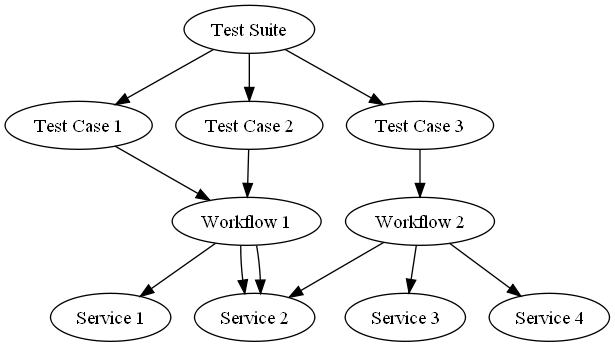
\includegraphics[scale=0.6]{test_tree.png}
	\caption{L'arbre de test}
	\label{TestTreeFig}
\end{figure}

L'arbre des tests est complètement retranscrit dans mon code. Chacun des types
d'objet correspond à une classe. Cependant j'ai conçu ces classes afin que 
l'arbre puisse devenir plus complexe. Ainsi toutes ces classes implémentent
l'interface \verb|Test|, ou l'interface \verb|TestSuite|, qui hérite de 
\verb|Test|. Ces deux interfaces se présentent ainsi (pour la description des 
interfaces \verb|Context| et \verb|Result| qui apparaissent \verb|Test|, voir 
partie \ref{NewAPI}) :

\begin{verbatim}
/**
 * The root interface for all of the test objects.
 * @author Hugo Wood
 */
public interface Test extends Runnable {
  
  /**
   * Returns the context of the test. The context acts as the input value of 
   * the run method and therefore should not be null before the {@link run} 
   * method is called.
   */
  Context getContext();

  /**
   * Returns the result of the test. The result acts as the output value of 
   * the run method and therefore should not be null after the {@link run} 
   * method has been called.
   */
  Result getResult();
   
}

/**
 * A test that contains other tests.
 * @author Hugo Wood
 */
public interface TestSuite extends Test, Iterable<Test> {
  
  /**
   * Returns the number of tests in this suite.
   */
  int getSize();

}
\end{verbatim}

Par conséquent, un service est un test, et un workflow une test suite. 
L'extensibilité vient du fait que via ce système d'interface, différentes 
implémentations peuvent cohabiter. Et c'est déjà le cas dans mon code puisque 
les classes \verb|SequentialTestSuite| (test suite qui exécutent ses tests en 
série) et \verb|ParallelTestSuite| (en parallèle) sont bien deux implémentations
différentes de \verb|TestSuite|. Un diagramme des classes simplifié de TCtest 5 
(la version que j'ai laissé en partant) est présenté en figure \ref{Classes}.
Notons en passant que \verb|Test| hérite de \verb|Runnable|, ce qui rend les 
objets de l'arbre facilement utilisables avec l'API \verb|java.util.concurrent| 
pour le multi-threading.

\begin{figure}[htb]
	\centering
	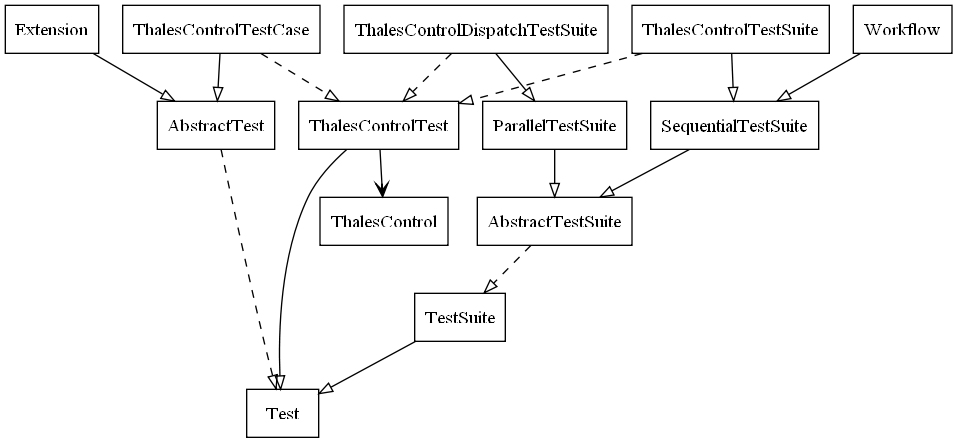
\includegraphics[scale=0.4]{classes.png}
	\caption{Diagramme des classes}
	\label{Classes}
\end{figure}

A \verb|Test| et \verb|TestSuite| vient s'ajouter l'interface 
\verb|ThalesControlTest| qui est simplement un test qui contient un objet de 
type \verb|ThalesControl|. On devine le rôle de chaque classe avec son nom et 
les classes dont elle hérite (mise à part \verb|ThalesControlDispathTestSuite|, 
décrite en \ref{ReParallel}).

\subsection{Reparallélisation}
\label{ReParallel}

Comme décrit en \ref{Parallel}, TCtest 1.0 est une application multi-threadée.
Cependant la parallélisation n'est pas optimale. En effet, elle n'autorise 
qu'un seul test à la fois, alors que la véritable contrainte est que l'on ne 
peut exécuter qu'un seul test à la fois \textit{par instance de ThalesControl}. 
J'ai donc écrit la classe \verb|ThalesControlDispathTestSuite| (voir le 
diagramme des classes en \ref{TestTree}). Les instances de cette classe 
analysent entièrement à l'avance l'ensemble 
des tests qu'elles ont à effectuer, déterminent les instances de ThalesControl qui 
vont être utilisées, créent un thread par instance, et enfin distribuent
les tests sur les différents thread suivant l'instance à laquelle ils sont 
destinés. L'avantage de cette méthode, outre son efficacité, est que son 
implémentation ne requiert pas de communications entre les threads. Le programme 
est donc bien plus robuste.

\subsection{Protection contre une configuration mal-formée}

TCtest 1.0 ne se protégeait quasiment pas contre des fichiers de configuration 
mal-formés. Comme j'avais standardisé tous les fichiers de configuration en 
les écrivant au format XML et utilisant JAXB pour les exploiter, j'ai pu 
centraliser dans une seule classe le code permettant de transformer une fichier 
XML en un objet complet avec comportement. Concrètement cette classe lit 
les fichiers de configuration avec JAXB, en tire des pseudo-objets réprésentant 
le contenu des fichiers, vérifie que ce contenu est valide, puis construit à 
partir du contenu des instances des classes de l'arbre de test, notemment des 
instances de \verb|ThalesContrlol|, \verb|ThalesControlTestCase|, 
\verb|Workflow| et \verb|ThalesControlDispatchTestSuite|.

En cas d'erreur dans l'étape de vérification, un message d'erreur est envoyé à 
l'utilisateur avec suffisamment de détails pour qu'il puisse corriger le fichier
de configuration incriminé.

\subsection{Manuel utilisateur}

J'ai écrit un manuel complet pour l'utilisateur de TCtest. Il en décrit le 
principe, comment en tirer parti ainsi que la manière dont les fonctionnalités
peuvent être étendues. Comme toute documentation produite par Thales CST, le 
manuel est écrit en Anglais. Une copie se trouve en annexe.
\newpage

\section{Conclusion}

Ce stage m'a apporté la confirmation que "l'informatique pour l'informatique" 
est la voie dans laquelle je veux m'engager. J'ai été plongé dans un 
environnement très technique que je ne connaissais que de très loin : 
l'intégration continue, Hudson, Sonar, Maven... Je connaissais peu, 
voire pas du tout ces outils. J'ai adoré apprendre à les utiliser et ai été très 
agréablement surpris de l'immensité de l'écosystème Java et de son fort 
penchant pour l'open-source. L'intégration continue m'a également beaucoup 
intéressé (j'ai installé Jenkins et Sonar sur ma propre machine).

La technique mise à part, l'environnement de travail était très agréable. 
Mes collègues étaient toujours disponibles pour m'aider à apprivoiser tous les 
nouveaux concepts que j'ai rencontré. J'ai apprécié travailler de pair avec un 
autre stagiaire. Cela permet de confronter des idées et généralement de conclure
à une meilleure solution que lorsque l'on est seul. Etre deux nous a aussi 
permis de comprendre TCtest beaucoup plus rapidement, malgré le peu de 
documentation.
\newpage

\section{Bibliographie et ressources d'intérêt}

\begin{description}
	\item[Rapport de Francis Ngougo]{}
	\item[Thales]{http://www.thalesgroup.com}
	\item[Wikipedia]{http://www.wikipedia.org}
	\item[Hudson]{http://hudson-ci.org}
	\item[Jenkins]{http://jenkins-ci.org}
	\item[Sonar]{http://sonarsource.org}
	\item[JAXB]{http://jaxb.java.net}
	\item[Jersey]{http://jersey.java.net}
	\item[Apache DB DdlUtils]{http://db.apache.org/ddlutils}
\end{description}

\section{Annexe}
\subsection{Manuel utilisateur}

\end{document}